\documentclass[a4paper,12pt]{article}

%%% Работа с русским языком
\usepackage{cmap}					% поиск в PDF
\usepackage{mathtext} 				% русские буквы в фомулах
\usepackage[T2A]{fontenc}			% кодировка
\usepackage[utf8]{inputenc}			% кодировка исходного текста
\usepackage[english,russian]{babel}	% локализация и переносы

\usepackage{amsmath,amsfonts,amssymb,amsthm,mathtools} % AMS
\usepackage{icomma} % "Умная" запятая: $0,2$ --- число, $0, 2$ --- перечисление
\usepackage{graphicx}
\usepackage{fullpage}

\graphicspath{{img/}}

% Default fixed font does not support bold face
\DeclareFixedFont{\ttb}{T1}{txtt}{bx}{n}{12} % for bold
\DeclareFixedFont{\ttm}{T1}{txtt}{m}{n}{12}  % for normal

% Custom colors
\usepackage{color}
\definecolor{deepblue}{rgb}{0,0,0.5}
\definecolor{deepred}{rgb}{0.6,0,0}
\definecolor{deepgreen}{rgb}{0,0.5,0}

\usepackage{listings}

% Python style for highlighting
\newcommand\pythonstyle{\lstset{
language=Python,
basicstyle=\ttm,
otherkeywords={self},             % Add keywords here
keywordstyle=\ttb\color{deepblue},
emph={MyClass,__init__},          % Custom highlighting
emphstyle=\ttb\color{deepred},    % Custom highlighting style
stringstyle=\color{deepgreen},
frame=tb,                         % Any extra options here
showstringspaces=false            % 
}}


% Python environment
\lstnewenvironment{python}[1][]
{
\pythonstyle
\lstset{#1}
}
{}

% Python for external files
\newcommand\pythonexternal[2][]{{
\pythonstyle
\lstinputlisting[#1]{#2}}}

% Python for inline
\newcommand\pythoninline[1]{{\pythonstyle\lstinline!#1!}}


\begin{document}

\begin{titlepage}
\begin{center}
  
\includegraphics[scale=0.5]{label.jpg}\\
  \vspace{20pt}
  МИНОБРНАУКИ РОССИИ\\
      Федеральное государственное бюджетное образовательное учреждение\\
      высшего профессионального образования\\
    <<Московский государственный технический университет радиотехники,\\
    электроники и автоматики>>\\ 
    {\large МГТУ МИРЭА}\\
    \line(2,0){500}\\
    \vspace{10pt}
    {\large Факультет информационных технологий\\}
    \vspace{10pt}
    {\large Кафедра МОСИТ}
\end{center}

\vspace{60pt}
\begin{center}
  Лабораторная работа №3\\
  \vspace{10pt}
  <<Разработка юнит-тестов для лексического анализатора>>\\
  \vspace{10pt}
  по дисциплине <<Тестирование программного обеспечения>>
\end{center}
\vspace{\fill}
Выполнил: \hfill студенты группы ИТО-1-10 Егоров А.Е.\\
\text{} \hfill Кулёв П.С.\\
\\
Преподаватель: \hfill Басок Б.М.
\begin{center}
\vspace{\fill}
Москва\\2014
\end{center}
\end{titlepage}

\newpage

\section{Постановка задачи}
\par Необходимо разработать программу на языке высокого уровня для тестирования лексического анализатора, входящего в состав интерпретатора простого языка.
\section{Задание}
\par Написать лексический анализатор (лексер), который принимает на вход исходный код программы и возвращает список токенов. Токен состоит из выражения на ЯП и тэга(класс токена). Для проверки принадлежности синтаксических конструкций синтаксису языка используется язык регулярных выражений.
\section{Практическая часть}

\subsection{Разработка лексического анализатора}
\par Для выполнения задания использовалась среда \verb|JetBrains PyCharm Community| \\ \verb|Edition V3.1| и интерпретатор языка \verb|Python v3.4.0.|\\

\par Сначала разработаем лексический анализатор согласно заданию, а затем протестируем его.

Для лексера нам потребуются стандартные модули:
\begin{itemize}
\item \verb|re| --- библиотека для работы с регулярными выражениями
\item \verb|sys| --- библиотека для работы с интерпретатором \verb|Python|\\
\end{itemize} 

Подключим их:
\begin{python}
import re
import sys\\
\end{python}
\vspace{12pt}

\par Определим основную (и единственную) функцию, которая будет делать всю работу (\pythoninline{lex(source, token_exprs)}), установим начальные значения для текущей позиции, списка токенов, которые мы будем заполнять и вернём в конце работы функции, а также позицию конца строки:

\begin{python}
def lex(source, token_exprs):
    pos = 0
    tokens = []
    end = len(source)
\end{python}

\vspace{12pt}

Лексер по очереди применяет каждое определённое нами регулярное выражение
к тексту начиная с текущей позиции \verb|pos|. 
\par Если есть совпадение, то лексер запоминает текст, который совпал (группа) и если в принятом наборе правил для этого выражения есть тэг, то лексер записывает тег и выражение в результирующий список; если совпадения нет, то лексер выдаёт ошибку и записывает в \verb|stderr| сообщение \verb|Illegal character| с указанием символа вызвавшего ошибку и завершает работу с кодом ошибки $1$. 
\par После успешного распознавания выражения счётчику текущей позиции присваивается позиция конца распознанной строки.
\par После обработки исходного текста функция возвращает список токенов.

Полный код лексера:
\begin{python}
import re
import sys


def lex(source, token_exprs):
    pos = 0
    tokens = []
    end = len(source)
    while pos < end:
        match = None
        for token_expr in token_exprs:
            pattern, tag = token_expr
            regex = re.compile(pattern)
            match = regex.match(source, pos)
            if match:
                text = match.group(0)
                if tag:
                    token = (text, tag)
                    tokens.append(token)
                break
        if not match:
            sys.stderr.write('Illegal character {s}'.format(
                                                 source[pos]))
            sys.exit(1)
        else:
            pos = match.end(0)
    return tokens
\end{python}
\vspace{12pt}

\newpage

\subsection{Разработка юнит-тестов}

\par Создадим новый Python файл, в котором определим базовые классы токенов и соответствия синтаксических конструкций классам токенов, а так же тестовые случаи для лексера. 
\par Использовать будем модуль \verb|unittest| из стандартной библиотеки.\\

Определим базовые классы:
\begin{itemize}
\item \verb|KEYWORD| --- для служебных слов языка
\item \verb|INT| --- для целых чисел
\item \verb|ID| --- для идентификаторов переменных\\
\end{itemize}

Определим с помощью регулярных выражений выражения языка, соответствующие нашим классам токенов:
\begin{python}
token_exprs = [
    (r'[ \t\n]+', None),
    (r'#[^\n]*', None),
    (r'keyword', KEYWORD),
    (r'[0-9]+', INT),
    (r'[A-Za-z][A-Za-z0-9_]*', ID)
]
\end{python}
\vspace{12pt}

\par Первое регулярное выражение определяет пробелы, табы и переносы строки. Класс токена не указан, поэтому будет просто игнорироваться лексером и не попадёт в парсер.
\par Второе выражение определяет комментарии, которые также не попадут в парсер.

\par Для того чтобы сделать новый юнит-тест, унаследуем класс \verb|unittest.TestCase| и опишем в нём методы, начинающиеся с \verb|_test|, в которых будем вызвать метафункцию \verb|lexer_test|, вызывающую функцию \verb|lex| с переданными ей параметрами.\\

\newpage

Листинг:\\ 
\begin{python}
import unittest
from lexer import *

KEYWORD = 'KEYWORD'
INT = 'INT'
ID = 'ID'

token_exprs = [
    (r'[ \t\n]+', None),
    (r'#[^\n]*', None),
    (r'keyword', KEYWORD),
    (r'[0-9]+', INT),
    (r'[A-Za-z][A-Za-z0-9_]*', ID)
]


class TestLexer(unittest.TestCase):
    def lexer_test(self, code, expected):
        actual = lex(code, token_exprs)
        self.assertEquals(expected, actual)

    def test_empty(self):
        self.lexer_test('', [])

    def test_id(self):
        self.lexer_test('abc', [('abc', ID)])

    def test_keyword_first(self):
        self.lexer_test('keyword', [('keyword', KEYWORD)])

    def test_space(self):
        self.lexer_test(' ', [])

    def test_id_space(self):
        self.lexer_test('abc def', [('abc', ID), ('def', ID)])


if __name__ == '__main__':
    test_names = ['test_lexer']
    suite = unittest.defaultTestLoader.loadTestsFromNames(test_names)
    result = unittest.TextTestRunner().run(suite)
\end{python}

\newpage

\par После описания всех тестовых случаев запустим их на выполнение и посмотрим результат. \\

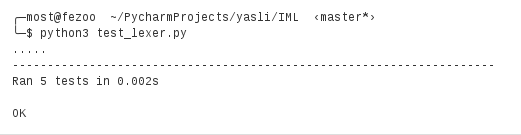
\includegraphics{passed1.png}

\par Все тесты завершены успешно. \\
Попробуем сымитировать ошибку изменив \pythoninline{self.lexer_test(' ', [])} на  \\ \pythoninline{self.lexer_test('vfds fds ', [])}

Посмотрим результат:

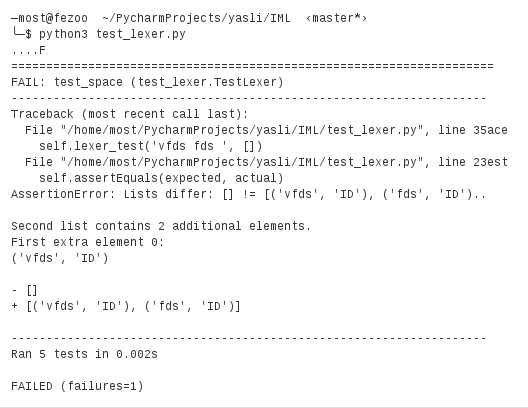
\includegraphics{failed1.png}

\newpage

\par По выводу видно где произошла ошибка. Вместо ожидаемого пустого списка (пробелы опускаются) из лексера вернулся список из двух токенов. К счастью, очевидно, что это не ошибка лексера.

Есть утилита \verb|coverage| для оценки покрытия \verb|Python| кода тестами.
Проверим покрытие:

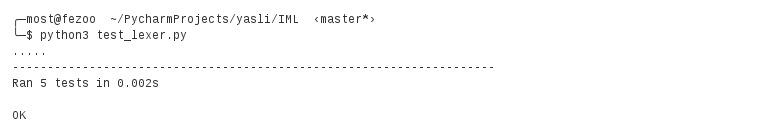
\includegraphics{coverage.png}

\end{document}